\section{The Software Technology}
\label{sec:background}


Apache Spark is an open-source distributed general-purpose cluster-computing framework. Spark provides an interface for programming entire clusters with implicit data parallelism and fault tolerance. Originally developed at the University of California, Berkeley's AMPLab, the Spark codebase was later donated to the Apache Software Foundation, which has maintained it since then. It is based on a data computing and analytics system based on Hadoop Map Reduce.

The official web defines Apache Spark as an unified analytics engine for large-scale data processing.\cite{sparkWebsite} \\*

Apache Spark has as its architectural foundation the resilient distributed dataset (RDD), a read-only multiset of data items distributed over a cluster of machines, that is maintained in a fault-tolerant way.\cite{brown:zaharia2010spark} The Dataframe API was released as an abstraction on top of the RDD, followed by the Dataset API. In Spark 1.x, the RDD was the primary application programming interface (API), but as of Spark 2.x use of the Dataset API is encouraged \cite{brown:eadline2015hadoop} even though the RDD API is not deprecated The RDD technology still underlies the Dataset API.\\*

It works in memory, which results in a much faster processing speed, it allows you to work on disk with large amount of data. In this way if we have a very large file or a quantity of information that does not fit in memory, the tool allows to store part in disk, which makes lose speed. This means that we have to try to find the balance between what is stored in memory and what is stored in disk, to have a satisfying speed and at the same time make  the total cost possibly the lowest, as the memory is always much more expensive than the disk.\\*

Spark and its RDDs were developed in 2012 in response to limitations in the MapReduce cluster computing paradigm, which forces a particular linear dataflow structure on distributed programs: MapReduce programs read input data from disk, map a function across the data, reduce the results of the map, and store reduction results on disk. Spark's RDDs function as a working set for distributed programs that offers a (deliberately) restricted form of distributed shared memory.\cite{zaharia2012resilient} \\*

Spark facilitates the implementation of both iterative algorithms, which visit their data set multiple times in a loop, and interactive/exploratory data analysis, i.e., the repeated database-style querying of data. The latency of such applications may be reduced by several orders of magnitude compared to Apache Hadoop MapReduce implementation Among the class of iterative algorithms are the training algorithms for machine learning systems, which formed the initial impetus for developing Apache Spark. \\*

Apache Spark requires a cluster manager and a distributed storage system. For cluster management, Spark supports standalone (native Spark cluster, where you can launch a cluster either manually or use the launch scripts provided by the install package. It is also possible to run these daemons on a single machine for testing), Hadoop YARN, Apache Mesos or Kubernetes. For distributed storage, Spark can interface with a wide variety, including Alluxio, Hadoop Distributed File System (HDFS), MapR File System (MapR-FS), Cassandra, OpenStack Swift, Amazon S3, Kudu, Lustre file system, or a custom solution can be implemented. Spark also supports a pseudo-distributed local mode, usually used only for development or testing purposes, where distributed storage is not required and the local file system can be used instead; in such a scenario, Spark is run on a single machine with one executor per CPU core.\cite{wang2014characterization} \\*

The friendly APIs, which Apache Spark provides, natively supports Java, Scala, R, and Python, giving you a variety of languages for building your applications. These APIs make it easy for developers, because they hide the complexity of distributed processing behind simple, high-level operators that lowers the amount of code required.\\*

It allows real time processing, with a module called Spark Streaming, which combined with Spark SQL will allows to process the data in the real time. As we are injecting the data, we can transform them and turn them to a final result.
Resilient Distributed Dataset (RDD), it uses the lazy evaluation, which means that all the transformations that we are carrying out on the RDD, are not resolved, but are stored in a directed acyclic graph (DAG), and when we execute an action, when the tool does not have more option than to execute all the transformations, that's when they are executed. This is a double-edged sword, as it has an advantage and a disadvantage. The advantage is that you gain speed by not making transformations continuously, but only when necessary. The disadvantage is that if some transformation raises some kind of exception, it will not be detected until the action is executed, so it is more difficult to program or debug something.

\subsection{Spark Architecture}

The main components that make up the framework are the following ones:

\begin{description}

	\item[Spark Core]: It is the base or set of libraries where the rest of modules are supported, is the core of the framework. It is also a shelter to API, that contains the backbone of Spark, that is RDDs (resilient distributed datasets). The basic functionality of Spark is present in Spark Core like:
	\begin{enumerate}
		\item Memory management
		\item Fault recovery
		\item Interaction with the storage system.
		\item It is in charge of essential I/O functionalities like:
		\begin{itemize}
			\item Programming and observing the role of Spark cluster
			\item Task dispatching
			\item Fault recovery
			\item It overcomes the snag of MapReduce by using in-memory computation.\\*
		\end{itemize}
	\end{enumerate}

	

	
	
	\item[Spark SQL]: It is the module for the processing of structured and semi-structured data. With this module we will be able to transform and perform operations on RDD or dataframes. It is designed exclusively for data processing.\\*
	
	
	\item[Spark Streaming]: It is the one that allows ingesting the data in real time. If we have a source, for example Kafka or Twitter, with this module we can ingest data from that source and dump them to a destination. Between the ingestion of data and its subsequent dump, we can have a series of transformations.\\*
	
	
	\item[Spark MLLib]: It is a very complete library that contains numerous Machine Learning algorithms, both clustering, classification, regression, and so on. It allows us, in a friendly way, to use Machine Learning algorithms.
	
	
	\item[Spark Graph]: It allows the processing of graphs (DAG). It does not allow to paint graphs, but it allows to create operations with graphs, with their nodes and edges, and to make operations.\\*
	
\end{description}


\begin{figure}[H]
	\centering
	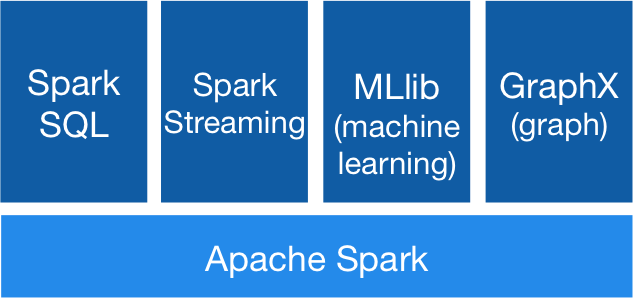
\includegraphics[scale=0.65]{figs/spark-components.png}
	\caption{Components of Apache Spark}Spark
	\label{fig:components-spark}
\end{figure}

\subsection{MLlib}

MLIB is part of Spark APIs which is interoperable with Python NumPy as well as with R-libraries. Implemented with Spark it is possible to use any type of data from any source or from the Hadoop platform such as HDFS, HBase, related database data sources or local data sources such as text documents.
Spark excels in iterative calculation processes allowing the processes written in the MLlib libraries to be executed quickly allowing their use and above all at an industrial level.\\*
MLlib provides many types of algorithms, as well as numerous useful functions. ML includes classification algorithms, regression, decision trees, recommendation algorithms, grouping. Among the most used utilities can include the characteristics of transformations, standardization and normalization, statistical functions and linear algebra.\\*

\subsection{Clustering}



Apache Spark can be configured to run on distributed mode on the cluster as a master node or slave node. Its master/slave architecture is composed by many main daemons and a cluster manager. T schedules and divides resource in the host machine which forms the cluster. 
\begin{itemize}

	\item Master Daemon — (Master/Driver Process)
	\item Worker Daemon –(Slave Process)
	\item Cluster Manager. Schedules and divides resources in the host machine which forms the cluster
\end{itemize}

As we can see in the figure~\ref{fig:clusters-spark} .
\begin{figure}[H]
	\centering
	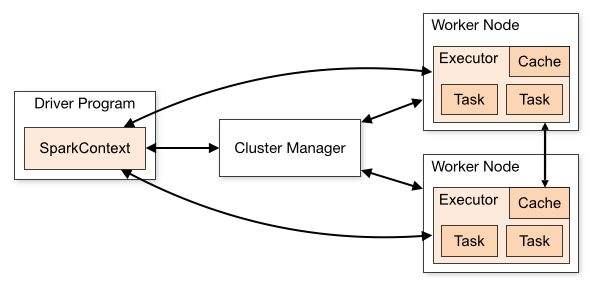
\includegraphics[scale=0.5]{figs/cluster-overview.png}
	\caption{Cluster management of Apache Spark}
	\label{fig:clusters-spark}
\end{figure}

